\chapter{System Design}
\begin{spacing}{1}
\setlength{\parskip}{0.3in}
\graphicspath{{./Chapter4/}}

\section{Introduction}
A system design refers to designing how the whole operations or system of an organization will run.There are certain functional and nonfunctional requirements in a system design that need to be fulfilled. It includes technical components, modules, architectures, different instructions, forms of inputs and outputs.

When designing a system we should keep in mind a few points:
\begin{itemize}
	\item Consistency
	\item Estimation
	\item Hardware management
	\item Availability
	\item Reliability
	\item Performance
	\item Abstraction
\end{itemize}
According to Akash DTH system design should emphasize on current system problems and work on improving the current system design .There should be some activities for developing the system such as identifying the goals,decomposing the system, managing the data values , controlling software sections, hardware allocation etc. The system should be designed in such a way that it should benefit the organization and also satisfy the user. The systems design document(s) contain the basic architecture, modules, to be implemented and are also subjected to review by software quality control. The review procedure is similar to the products requirement review and the procedure itself with supporting documentation should be documented in the organization’s standards library.

\section{Objective}
Main Objective of any system design is to produce a model of System.  Akash DTH focuses on following objectives to design a comfortable model for their system.
\begin{enumerate}
	\item \textbf{Practicality} \newline The systems must be stable \& can be operated by people with average intelligence. Because There are a huge number of low educated service workers who cooperate with  officers every hour. 
	\item \textbf{Correctness}  \newline The design should be correct as per the requirements and both customers and employees can be beneficial from  system.
	\item \textbf{Completeness} \newline  The design should have all the components like data structures, modules, external interfaces etc.
	\item \textbf{Efficiency} \newline  Expensive \& scarce resources should be used efficiently by the system.
\end{enumerate}

\section{Structure Design}
Structured systems analysis and design  is a set of standards for systems analysis and application design. It uses a formal methodical approach to the analysis and design of information systems. It was developed by Learmonth Burchett Management Systems (LBMS) and the Central Computer Telecommunications Agency (CCTA) in 1980-1981 as a standard for developing British database projects.It follows the waterfall life cycle model starting from the feasibility study to the physical design stage of development. One of the main features of Structure Analysis is the intensive user involvement in the requirements analysis stage. The users are made to sign off each stage as they are completed assuring that requirements are met. The users are provided with clear, easily understandable documentation consisting of various diagrammatic representations of the system.In Akash DTH Structure design the main focus was the users or customers of the DTH service. 

\subsection{Data Flow Diagram (DFD)}
A Data Flow Diagram (DFD) is a graphical representation of the “flow” of data through an information system , modeling its process aspects. Often it is a preliminary step used to create an overview of the system that can later be elaborated. DFDs can also be used for the visualization of data processing (structured design) and show what kind of information will be input to and output from the system, where the data will come from and go to, and where the data will be stored. It does not show information about the timing of processes or information about whether processes will operate in sequence or in parallel. In the process of Akash DFD everything was taken into consideration , we proposed four DFD in their existing system.Akash DTH previous  DFD was good but that they could not satisfy customer requirements and it was very difficult to cooperate with every level of employees so we proposed  some advanced dfd’s to satisfy every type of requirements and which will cost beneficial for their company.

\subsubsection{DFD of the Proposed Customer Service }
There are some big lacking in their previous customer service dfd. It was very hard to to add a new customer in their previous DFD system. Customer need to register from their local retailer point physically. So in the present pandemic situation it is very hard to add a new customer. And the customer service procedure was a big hazard for the customers. They needed to call the local retailer for their every problem and wait for service-serial. 

\begin{figure}[H]
	\centering
	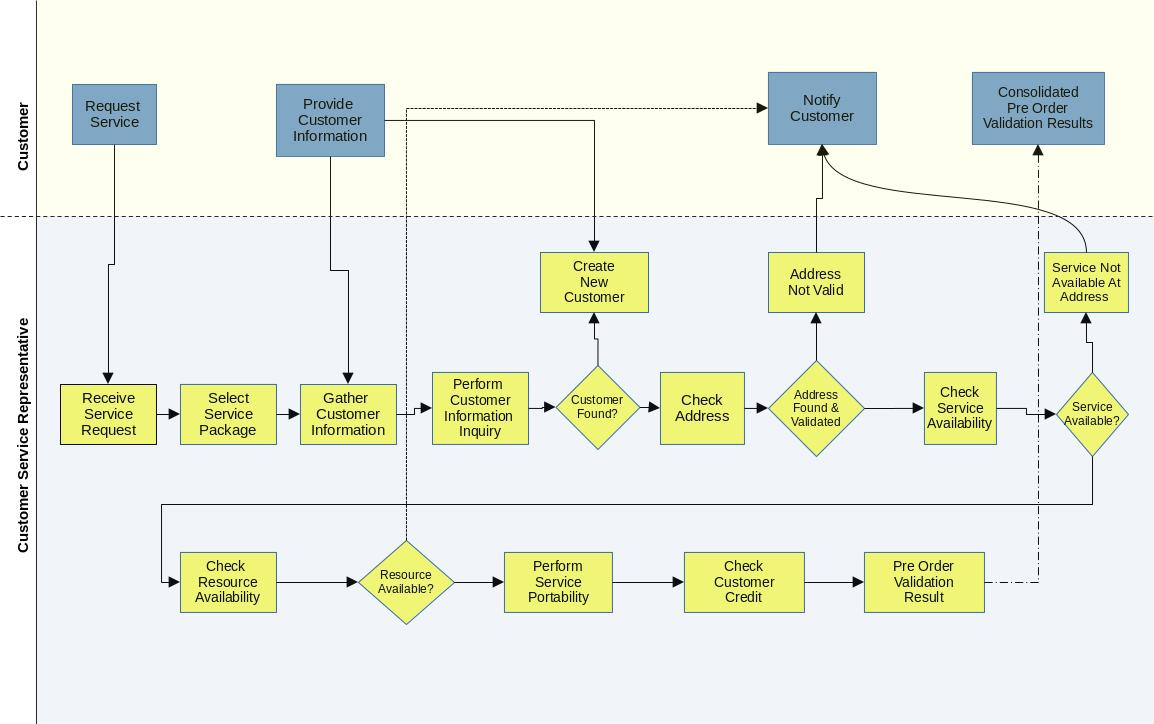
\includegraphics[width=0.8\textwidth]{flow22}
	\caption{Customer Service DFD}
	\label{fig:dfdproposed1}
\end{figure}

In this proposed customer service, customers can request a new connection directly from online and the initial papers of the customer can be validated by an authorized sells representative. If the customers address is valid for selected service and all others resources are available then customer will get a conformed notification about the their new connection and local service representative will get notified about new customer connection and will provide all necessary services as soon as possible.  If it is not possible to provide new connection due to resource scarcity or unavailability at customers location then customer will get notified about these problems immediately. This new model will bring all the customers needs under a single roof. 

\subsubsection{DFD of the  Log In System}
For the previously proposed customer service DFD there will need a login system.Log in system is the most valuable part of Customer Service , to identify a customer or to register a customer login System is essential. The previous retailer phone call service was a big factor of customer dissatisfaction.

\begin{figure}[H]
	\centering
	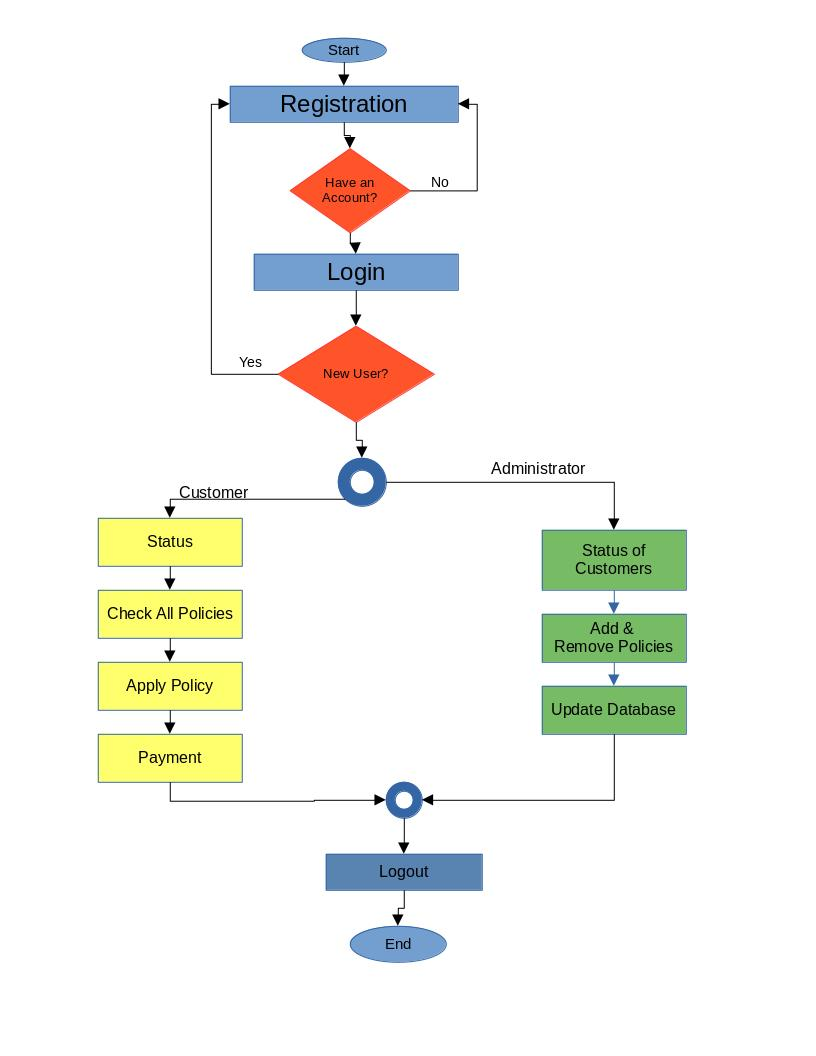
\includegraphics[width=0.8\textwidth]{activity}
	\caption{User Login DFD}
	\label{fig:dfdproposed2}
\end{figure}

In this new proposed user login system, customers can now login directly and can check his/her service status, can view all other provided policies and add or remove policies, can view the current monthly bill and also pay the bill directly from proposed integrated payment gateway. All the authorized admin and customers will use the same the gateway for login purpose but their actions will fully isolated as the new permission policy applied in user level. So there is no risk regarding information leakage or unauthorized  access.

\subsection{Structure English}
Structure English provides a further simplified and also precised description of a system aiming to get benefit of both programming logic and natural language. With using it both the system developer can express the system's working logic and the business analyst can overview the business structure and cost and profit analysis, and both team can communicate and cooperate in much a robust way.  
\subsubsection{Package Customization Policy}
From a DTH service provider, it will be a great marketing strategy and also profitable idea if they give the user the right to choose what channels will they subscribe and paid for. With three categorical plans, all users will by default be part of the basic plan and charge the minimum monthly subscription fee. But the user can add the channels to their subscription list and according to the number of channels he subscribed along with number of subscribed HD channels customer category will change dynamically and the customer will pay only the fees according to his additional subscription.

The package customization module consists of two sub procedures, \textbf{addChannel} and \textbf{removeChannel}. The pseudo code for user package customization is given below:

	\begin{algorithm}
	\caption{Add channel to user package}\label{add}
	\begin{algorithmic}[1]
		\Procedure{addChannel}{customer, channel}
		\State $\textit{customer.subscriptionList.add(channel)}$
		\State $\textit{customer.totalSubscription} \gets \textit{customer.totalSubscription + 1} $
		\If {$\textit{channel.type} == \emph{HD}$}
		\State $\textit{customer.hdSubscription} \gets \textit{customer.hdSubscription + 1}$
		\EndIf
		\If {$\textit{customer.hdSubscription} > \emph{BasicHDLimit or }  \textit{customer.totalSubscription} > \emph{BasicCHLimit}$}
		\State $\textit{customer.type} \gets \emph{ADVANCE}$
		\State $\textit{extraSubs} \gets \textit{customer.totalSubscription} - \textit{BasicCHLimit}$
		\State $\textit{customer.monthlyBill}  \gets \textit{minRate} + (\textit{extraSubs} * \textit{advanceRate})$
		\ElsIf {$\textit{customer.hdSubscription} > \emph{AdvanceHDLimit } \emph{or } \textit{customer.totalSubscription} > \emph{AdvanceCHLimit}$}
		\State $\textit{customer.type} \gets \emph{PREMIUM}$
		\State $\textit{extraSubs} \gets \textit{customer.totalSubscription} - \textit{PremiumCHLimit}$
		\State $\textit{customer.monthlyBill}  \gets \textit{minRate} + (\textit{extraSubs} * \textit{premiumRate})$
		\Else
		\State $\textit{customer.type} \gets \emph{BASIC}$
		\State $\textit{customer.monthlyBill}  \gets \textit{minRate}$
		\EndIf
		\EndProcedure
	\end{algorithmic}
\end{algorithm}
\begin{algorithm}
	\caption{Remove channel from user package}\label{remove}
	\begin{algorithmic}[H]
		\Procedure{removeChannel}{customer, channel}
		\State $\textit{customer.subscriptionList.remove(channel)}$
		\State $\textit{customer.totalSubscription} \gets \textit{customer.totalSubscription - 1} $
		\If {$\textit{channel.type} == \emph{HD}$}
		\State $\textit{customer.hdSubscription} \gets \textit{customer.hdSubscription - 1}$
		\EndIf
		\If {$\textit{customer.hdSubscription} > \emph{BasicHDLimit or }  \textit{customer.totalSubscription} > \emph{BasicCHLimit}$}
		\State $\textit{customer.type} \gets \emph{ADVANCE}$
		\State $\textit{extraSubs} \gets \textit{customer.totalSubscription} - \textit{BasicCHLimit}$
		\State $\textit{customer.monthlyBill}  \gets \textit{minRate} + (\textit{extraSubs} * \textit{advanceRate})$
		\ElsIf {$\textit{customer.hdSubscription} > \emph{AdvanceHDLimit } \emph{or } \textit{customer.totalSubscription} > \emph{AdvanceCHLimit}$}
		\State $\textit{customer.type} \gets \emph{PREMIUM}$
		\State $\textit{extraSubs} \gets \textit{customer.totalSubscription} - \textit{PremiumCHLimit}$
		\State $\textit{customer.monthlyBill}  \gets \textit{minRate} + (\textit{extraSubs} * \textit{premiumRate})$
		\Else
		\State $\textit{customer.type} \gets \emph{BASIC}$
		\State $\textit{customer.monthlyBill}  \gets \textit{minRate}$
		\EndIf
		\EndProcedure
	\end{algorithmic}
\end{algorithm}   

\newpage
\subsection{Data Dictionary}
A data dictionary contains metadata , data about the customers \& employees. The data dictionary is very important as it contains information such as what is in the database, who is allowed to access it, where is the database physically stored etc. The users of the database normally don't interact with the data dictionary, it is only handled by the database administrators.
The Akash DTH data dictionary  contains information about the following:
\begin{itemize}
	\item Packages of channels. 
	\item Discount percentage for each package.
	\item Plans Payment Policy 
	\item Duration of Plan.
\end{itemize}
Data Dictionary mainly used for an overview of the database ,Here in Akash DTH a separate public Data Dictionary is visible in the website.The discount policy was modified slightly in consideration with customer satisfaction as well as cost efficient for Akash DTH business.A well maintained public discount policy can attract new customer’s.

\begin{figure}[H]
	\centering
	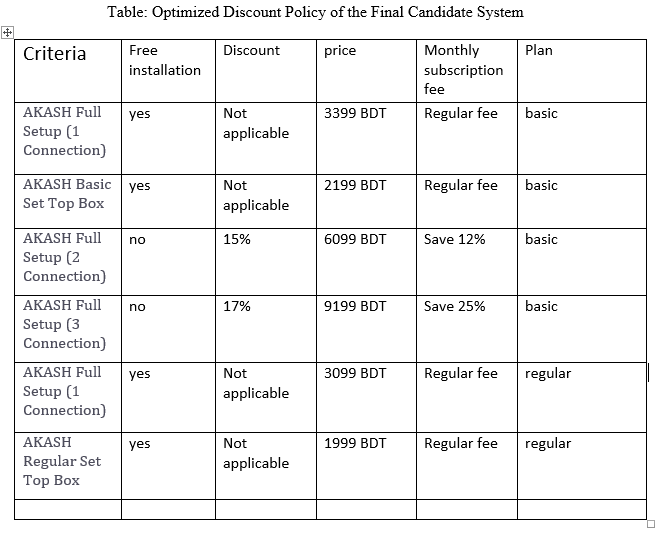
\includegraphics[width=0.8\textwidth]{table}
	\caption{Optimized Discount Policy of the Final Candidate System}
	\label{fig:table41}
\end{figure}

That Discount policy is satisfying for customer requirements as Akash DTH can earn a smart amount from every customer.Here, in our proposed discount model, the consistency is monitored on account of customer satisfaction as well as considering company benefits.

\section{Database Design}
Data storage is considered by some to be the heart of an information system. First, the data has to be available when the user wants to use them. Second, the data must be accurate and consistent (they must possess integrity). Beyond this requirement, the objectives of database design include efficient storage of data as well as efficient updating and retrieval. Finally, it is necessary that information retrieval be purposeful.The information obtained from the stored data must be in a form useful for managing, planning, controlling, or decision making.There are two approaches to the storage of data in a computer-based system. The first is to store the data in individual files, each unique to a particular application. The second approach involves building a database.A database is a formally defined and centrally controlled store of data intended for use in many different applications.
In Akash DTH customer files are often designed only with immediate needs in mind, so it becomes important to query the system for a combination of some of the attributes, these attributes may be contained in separate files or may not even exist. Databases are planned, so that data is organized for efficient storage and effective retrieval. In the database design process of Akash DTH, first of all we focused on their existing active  module’s. We seperate those module’s according to activities. Before designing the whole database first we design a class management system diagram or class diagram of Akash DTH.

\subsection{Akash DTH Management System Class Diagram}
Class diagrams are the blueprints of your system or subsystem. You can use class diagrams to model the objects that make up the system, to display the relationships between the objects, and to describe what those objects do and the services that they provide.

Akash DTH Management System Class diagram describes the official management system classes. Their attribute operation and relationship among objects. The main classes of Aakash DTH management systems are channels ,Customers, Users,Payment,Plans , Login.

\begin{figure}[H]
	\centering
	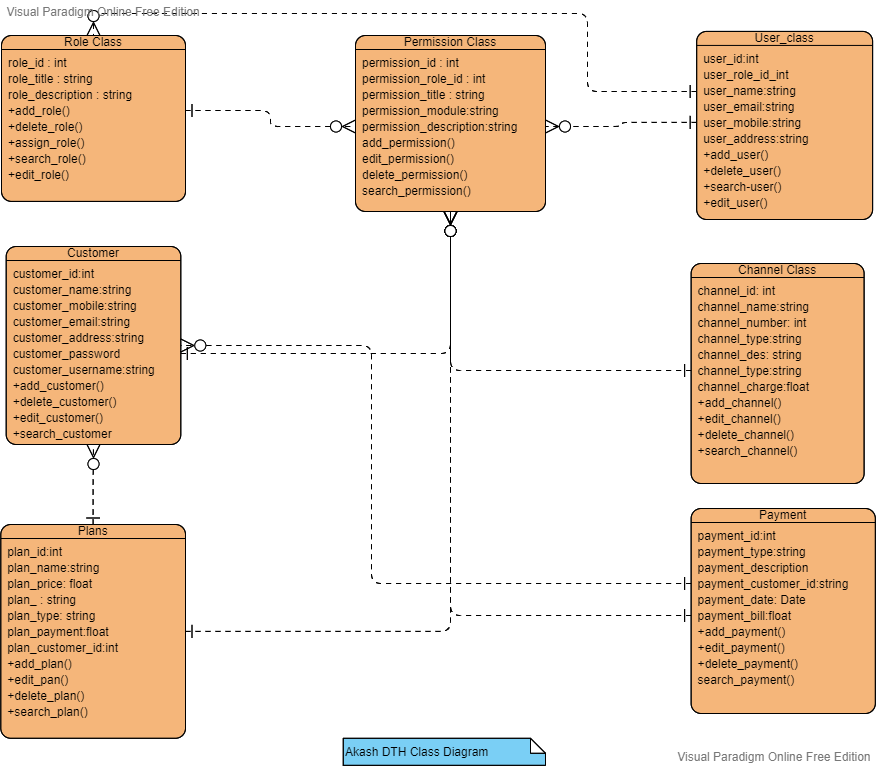
\includegraphics[width=0.8\textwidth]{classDiagram}
	\caption{Akash DTH class diagram}
	\label{fig:classdiagram}
\end{figure}

Here the visual representation of all the classes and their relationship. The heart of the class diagram is the permission class , all the other classes depend on the permission class. The relationships are described in the diagram.We mainly found out the attribute and relationship among the classes and functionality of each class.

\subsection{ER Diagram}
An ER diagram is a means of visualizing how the information a system produces is related. There are five main components of an ERD:
\newline
\textbf{Entities}: which are represented by rectangles. An entity is an object or concept about which you want to store information.
\begin{figure}[H]
	\centering
	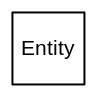
\includegraphics{entity}
	\label{fig:entity}
\end{figure}
\textbf{Weak Entities}: A weak entity is an entity that must be defined by a foreign key relationship with another entity as it cannot be uniquely identified by its own attributes alone.
\begin{figure}[H]
	\centering
	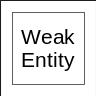
\includegraphics{weak}
	\label{fig:weakentity}
\end{figure}
\textbf{Actions}: which are represented by diamond shapes, show how two entities share information in the database.
\begin{figure}[H]
	\centering
	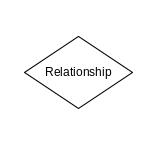
\includegraphics{relatio}
	\label{fig:relation}
\end{figure}
\textbf{Attributes}: which are represented by ovals. A key attribute is the unique, distinguishing characteristic of the entity. For example, an employee's social security number might be the employee's key attribute
\begin{figure}[H]
	\centering
	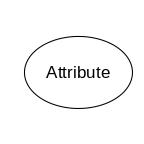
\includegraphics{attribute}
	\label{fig:attribute}
\end{figure}

\subsubsection{ER Diagram of Akash DTH}
The ER diagram represents the model of Akash DTH management system entity. The Entity relationship diagram of Akash DTH management system shows all the visual representation of database tables and relation between customer, payment ,login etc. It used structure data to define the relationships between structure data groups of Akash DTH system functionalities.The Main Entities of Akash DTH are

\begin{itemize}
	\item User
	\item Login
	\item Role
	\item Permission
	\item Plan
	\item Channels
	\item Customers
\end{itemize}

\begin{figure}[H]
	\centering
	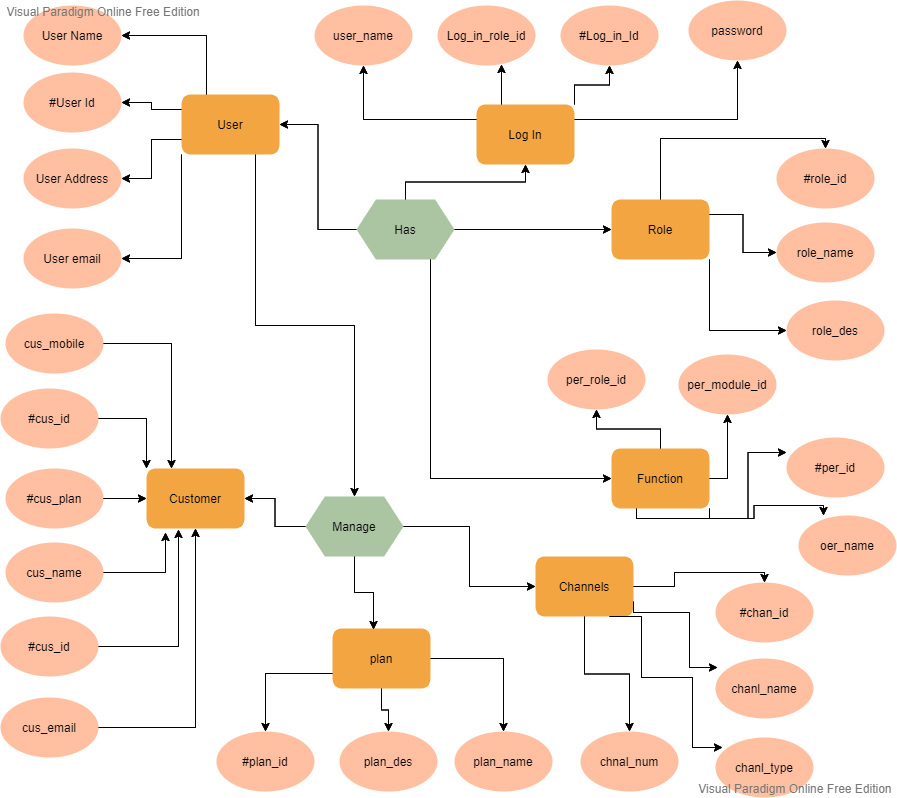
\includegraphics[width=0.8\textwidth]{ER}
	\caption{ER diagram for Akash DTH}
	\label{fig:er}
\end{figure}

The Manage and Has are relationship entities , the Has entity relation mainly a combination of user,login,role and permission entity and decide their access availability of other entity classes.Manage relationship entity is a model for customers,plan and channels .

\section{Conclusion}
A systemic approach is required for a coherent and well-running system. Bottom-Up or Top-Down approach is required to take into account all related variables of the system. In our designing process we applied a Top-Down approach to define our Order Tracking model with a structured chart. Module cohesion and coupling are maintained in a generic way during explaining the particular system. A designer generally uses the modelling languages to express the information and knowledge in a structure of a system that is defined by a consistent set of rules and definitions., we presented the Maintenance and Discount Policies with the help of structured english and data dictionary which gives crystal clear concepts of how to apply the policies in a storming business race. A well-formed database design is important in ensuring consistent data, elimination of data redundancy, efficient execution of queries and high performance application. If the business grows and progresses in an extensive way in future, this model can be developed more on further market demand. 

\end{spacing}
\newpage
	